\section{Теория вероятностей}

Статистический вывод касается обучения на опыте: мы наблюдаем случайную выборку $\mathbf{x} = (x_1, x_2, \cdots, x_n)$ и хотим вывести свойства полной совокупности $\mathbf{X} = (X_1, X_2,\cdots, X_N)$, которая дала образец. Теория вероятностей идет в противоположном направлении: из состава популяции $\mathbf{X}$ мы выводим свойства случайной выборки $\mathbf{x}$ и статистики, вычисляемой по $\mathbf{x}$. Статистический вывод как математическая наука был разработан почти исключительно в терминах теории вероятностей. Здесь мы кратко рассмотрим некоторые фундаментальные концепции вероятности, включая распределения вероятностей, ожидания и независимость. 

В качестве первого примера пусть $x$ представляет результат броска правильной кости, поэтому $x$ с равной вероятностью будет 1, 2, 3, 4, 5 или 6. Мы запишем это в вероятностной нотации как 
\begin{equation}
    Prob\{x=k\}=1/6\qquad for\quad k=1,2,3,4,5,6.
\end{equation}

Случайное число, такое как $x$, часто называется случайной величиной. 

Вероятности - это идеализированные или теоретические пропорции. Мы можем представить себе пространство $\mathbf(U) = \{U_1 U_2, \cdots, U_N\}$ возможных бросков кубика, где $U_j$ полностью описывает физический акт j-го броска с соответствующими результатами $\mathbf{X} = (X_1, X_2,\cdots, X_N)$. Здесь $N$ может быть очень большим или даже бесконечным. Выражение $Prob\{x = 5\} = 1/6$ означает, что случайным образом выбранный член $\mathbf{X}$ имеет 1/6 шанс быть равным 5, или, проще говоря, 1/6 членов $\mathbf{X}$ равняется 5. Обратите внимание что такие вероятности, как пропорции, никогда не могут быть меньше 0 или больше 1. 

Для удобства обозначений определим частоты $f_k$, 
\begin{equation}
    f_k=Prob\{x=k\},
\end{equation}
так что у справедливой кости $f_k = 1/6$ для $k = 1, 2, \cdots, 6$. Распределение вероятностей случайной величины $x$, которую мы обозначим $F$, является любым полным описанием вероятностного поведения $x$. $F$ также называется распределением вероятностей популяции $\mathbf{X}$. Здесь мы можем взять $F$ как вектор частот 
\begin{equation}
    F=(f_1,f_2,\cdots,f_6)=(1/6, 1/6, \cdots,1/6).
\end{equation}
Несправедливым будет кубик, для которого $F$ не равно $(1/6, 1/6, \cdots,1/6)$. 

Некоторые распределения вероятностей возникают настолько часто, что получили специальные названия. Говорят, что случайная величина $x$ имеет биномиальное распределение с размером $n$ и вероятностью успеха $p$, что обозначается 
\begin{equation}
    x\sim Bi(n,p),
\end{equation}
если его частоты 
\begin{equation}
    f_k=C_n^kp^k(1-p)^{n-k}\quad for\quad k=0,1,2,\cdots,n.
\end{equation}
Здесь $n$ -- положительное целое число, $p$ -- число от 0 до 1, а $C_n^k$ -- биномиальный коэффициент $n! / [K! (n-k)!]$. На рисунке 3.2 показано распределение $F = (f_0, f_1, \cdots, f_n)$ для $x \sim Bi (n, p)$, при $n = 25$ и $p = 0.25, 0.50$ и $0.90$. Мы также пишем $F = Bi (n, p)$ для обозначения ситуации (3.4). 
\newline

\noindent
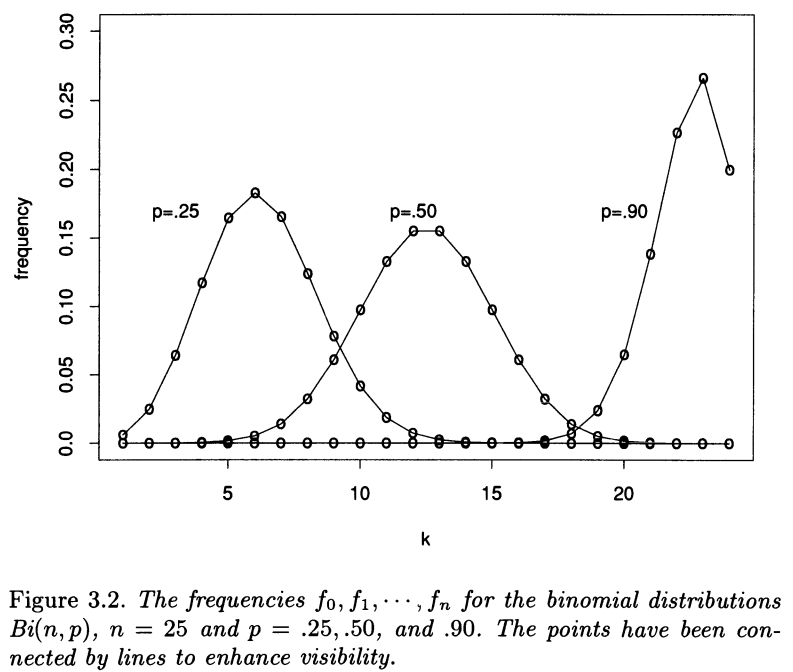
\includegraphics[width=\linewidth]{2/f32.png}
\newline

Пусть $A$ -- набор целых чисел. Тогда вероятность того, что $x$ принимает значение в $A$, или, проще говоря, вероятность $A$, равна 
\begin{equation}
    Prob\{x\in A\}=Prob\{A\}=\sum_{k\in A}f_k.
\end{equation}
Например, если $A = \{1, 3, 5, \cdots, 25\}$ и $x \sim Bi (25, p)$, то $Prob \{A\}$ -- это вероятность того, что биномиальная случайная величина размера 25 и вероятность успеха $p$ равно нечетному целому числу. Заметьте, что, поскольку $f_k$ -- это теоретическая доля раз, когда $x$ равно $k$, сумма $\sum_{k\in A}f_k = Prob \{A\}$ -- это теоретическая доля раз, когда $x$ принимает свое значение в $A$. 

Выборочное пространство $x$, обозначенное $S_x$, представляет собой набор возможных значений $x$. Для правильного кубика $S_x = \{1, 2, \cdots, 6\}$, а $S_x = \{0, 1, 2, \cdots, n\}$ для распределения $Bi (n, p)$. По определению $x$ встречается в $S_x$ каждый раз, то есть с теоретической пропорцией 1, поэтому
\begin{equation}
    Prob\{S_x\}=\sum_{k\in S_x}f_k=1.
\end{equation}
Для любого распределения вероятностей целых чисел частоты $f_j$ являются неотрицательными числами, сумма которых равна 1. 

В наших примерах до сих пор пространство выборки $S_x$ было подмножеством целых чисел. Одна из удобных особенностей вероятностных распределений заключается в том, что их можно определять в довольно общих пространствах. Рассмотрим данные юридического факультета на Рисунке 3.1. Мы могли бы принять $S_x$ за положительный квадрант плоскости
\begin{equation}
    S_x=\mathbf{R}^{2+}=\{(y,z),y>0,z>0\}.
\end{equation}
(Сюда входят такие значения, как $x = (10^6, 10^9)$, но не повредит, если $S_x$ будет слишком большим.) Для подмножества $A$ из $S_x$ мы все равно будем писать $Prob \{A\}$, чтобы указать вероятность того, что $x$ встречается в $A$. 

Например, мы могли бы взять 
\begin{equation}
    A=\{(y,z):0<y<600,0<z<3.0\}.
\end{equation}
Юридическая школа $x \in A$, если ее входной класс 1973 года имел LSAT менее 600 и средний балл менее 3,0. В этом случае мы знаем полную популяцию $\mathbf{X}$; это 82 точки, указанные на левой панели рисунка 3.1 и в таблице 3.2. Из них 16 находятся в $A$, поэтому 
\begin{equation}
    Prob\{A\}=16/82=0.195.
\end{equation}
Здесь идеализированная пропорция $Prob \{A\}$ -- это действительная пропорция. Только в тех случаях, когда у нас есть полная генеральная совокупность, можно напрямую оценить вероятности как пропорции. 

Распределение вероятностей $F$ $x$ по-прежнему определяется как полное описание вероятностей $x$. В примере с юридической школой $F$ можно описать следующим образом: для любого подмножества $A$ из $S_x = \mathbf{R}^{2+}$, 
\begin{equation}
    Prob\{x\in A\}=\#\{X_j\in A\}/82,
\end{equation}
где $\# \{X_j \in A\}$ -- это 82 точки на левой панели рисунка 3.1, которые лежат в $A$. Другим способом сказать, что $F$ -- это дискретное распределение, полагая вероятность (или частоту) 1/82 на каждую из указанных 82 точек. 

Вероятности можно определять непрерывно, а не дискретно, как в (3.6) или (3.11). Самый известный пример -- нормальное (или гауссово, или колоколообразное) распределение. Определено, что случайная величина $x$ с действительными значениями имеет нормальное распределение со средним $\mu$ и дисперсией $\sigma^2$, записанное 
\begin{equation}
    x\sim N(\mu,\sigma^2)\quad or \quad F=N(\mu,\sigma^2),
\end{equation}
если
\begin{equation}
    Prob\{x\in A\}=\int_A\frac{1}{\sqrt{2\pi\sigma^2}}\exp^{-\frac{1}{2}(\frac{x-\mu}{\sigma})^2}dx
\end{equation}
для любого подмножества $A$ действительной прямой $\mathbf{R}^1$. Интеграл в (3.13) берется по значениям $x \in A$. 

Существуют версии нормального распределения с более высокой размерностью, которые включают взятие интегралов, подобных (3.13), по многомерным множествам $A$. Нам не понадобятся непрерывные распределения для разработки бутстрепа. Как мы увидим, одним из основных стимулов для развития бутстрепа является желание заменить теоретические вычисления компьютерными с использованием специальных распределений. 

Математическое ожидание вещественной случайной величины $x$, обозначаемой $E(x)$, является ее средним значением, где среднее значение берется по возможным результатам $x$, взвешенным в соответствии с его распределением вероятностей $F$. Таким образом, 
\begin{equation}
    E(x)=\sum_{x=0}^nxC_n^xp^x(1-p)^x\quad for\quad x\sim Bi(n,p),
\end{equation}
и
\begin{equation}
    E(x)=\int_{-\infty}^\infty x\frac{1}{\sqrt{2\pi\sigma^2}}\exp^{-\frac{1}{2}(\frac{x-\mu}{\sigma})^2}dx\quad for \quad x\sim N(\mu,\sigma^2).
\end{equation}
Нетрудно показать, что $E(x) = np$ для $x \sim Bi (n, p)$ и $E (x) = \mu$ для $x \sim N (\mu, \sigma^2)$.

Иногда мы пишем математическое ожидание как $E_F (x)$, чтобы указать, что среднее значение берется по отношению к распределению $F$.

Предположим, что $r = g (x)$ -- некоторая функция случайной величины $x$. Тогда $E (r)$, математическое ожидание $r$, представляет собой теоретическое среднее значение $g (x)$, взвешенное в соответствии с распределением вероятности $x$. Например, если $x \sim  N (\mu, \sigma^2)$ и $r = x^3$, то 
\begin{equation}
    E(r)=\int_{-\infty}^\infty x^3\frac{1}{\sqrt{2\pi\sigma^2}}\exp^{-\frac{1}{2}(\frac{x-\mu}{\sigma})^2}dx.
\end{equation}

Вероятности -- это частный случай ожиданий. Пусть $A$ -- подмножество $S_x$, и возьмем $r = I_{\{x\in A\}}$, где $I_{\{x\in A\}}$ - индикаторная функция
\begin{equation}
    I_{\{x\in A\}}=\begin{cases}
      1\quad if \quad x\in A\\
      0\quad if \quad x\not\in A
    \end{cases}.
\end{equation}
Тогда $E(r)$ равна $Prob\{x\in A\}$ или 
\begin{equation}
    E(I_{\{x\in A\}})=Prob\{x\in A\}.
\end{equation}
Например, если $x\sim N(\mu, \sigma^2)$, тогда
\begin{equation}
    E(r)=\int_{-\infty}^\infty I_{\{x\in A\}}\frac{1}{\sqrt{2\pi\sigma^2}}\exp^{-\frac{1}{2}(\frac{x-\mu}{\sigma})^2}dx=
    \int_{A} \frac{1}{\sqrt{2\pi\sigma^2}}\exp^{-\frac{1}{2}(\frac{x-\mu}{\sigma})^2}dx,
\end{equation}
является $Prob\{x\in A\}$ в соответствии с (3.13).

Понятие математического ожидания как теоретического среднего является очень общим и включает случаи, когда случайная величина $x$ не является действительной. В ситуации с юридической школой, например, нас может заинтересовать математическое ожидание соотношения LSAT и GPA. Пусть $x = (y, z)$, как в (3.8), тогда $r = y/z$, и математическое ожидание $r$ равно 
\begin{equation}
    E(LSAT/GPA)=\frac{1}{82}\sum_{j=1}^82(y_j/z_j)
\end{equation}
где $x_j = (y_j, z_j)$ -- j-я точка в таблице 3.2. Численная оценка (3.20) дает $E(LSAT/GPA) = 190.8$. 

Пусть $\mu_x = E_F(x)$ для $x$ вещественной случайной величины с распределением $F$. Дисперсия $x$, обозначаемая $\sigma^2_x$ или просто $\sigma^2$, определяется как ожидаемое значение $y = (x- \mu)^2$. Другими словами, $\sigma^2$ -- это теоретический средний квадрат расстояния случайной величины $x$ от ее математического ожидания $\mu$, 
\begin{equation}
    \sigma^2_x = E_F(x-\mu_x)^2.
\end{equation}
Дисперсия $x\sim N (\mu, \sigma^2)$ равна $\sigma^2$; дисперсия $x\sim Bi (n, p)$ равна $np (1 - p)$. Стандартное отклонение случайной величины определяется как квадратный корень из ее дисперсии. 

Две случайные величины $y$ и $z$ называются независимыми, если 
\begin{equation}
    E[g(y)h(z)]=E[g(y)]E[h(z)]
\end{equation}
для всех функций $g(y)$ и $h(z)$. Независимость (3.22) подразумевает, что случайный результат $y$ не влияет на случайный результат $z$, и наоборот. 

Чтобы убедиться в этом, пусть $B$ и $C$ - подмножества $S_y$ и $S_z$ соответственно, выборочные пространства $y$ и $z$, а $g$ и $h$ - индикаторные функции $g(y) = I_{\{y\in B\}}$ и $h (z) = I_{\{z\in C\}}$ · Обратите внимание, что 
\begin{equation}
    I_{\{y\in B\}}I_{\{z\in C\}}=\begin{cases}
      1\quad if \quad y\in B\quad and\quad z\in C\\
      0\quad otherwise.
    \end{cases}
\end{equation}
Итак, $I_{\{y\in B\}}I_{\{z\in C}\}$ -- индикаторная функция пересечения ${\{y \in B\}} \cap {\{z \in C\}}$. Тогда в силу (3.18) и определения независимости (3.22) 
\begin{equation}
    \begin{array}{l}
        Prob\{(y,z)\in B\cap C\} = E(I_{\{y\in B\}}I_{\{z\in C\}})=\\ \\
        =E(I_{\{y\in B\}})E(I_{\{z\in C\}}) = Prob\{y\in B\}Prob\{z\in C\}.
    \end{array}
\end{equation}

Глядя на рисунок 3.1, мы видим, что (3.24) не выполняется для примера юридической школы, поэтому LSAT и GPA не являются независимыми. 

Независимо от того, независимы ли $y$ и $z$, ожидания подчиняются простому правилу сложения 
\begin{equation}
    E[g(y)+h(z)]=E[g(y)]+E[h(z)].
\end{equation}
В общем виде
\begin{equation}
    E[\sum_{i=1}^ng_i(x_i)]=\sum_{i=1}^nE[g_i(x_i)]
\end{equation}
для любых функций $g_i$ и любых $n$ случайных величин $x_1, x_2,\cdots, x_n$. 

Случайная выборка с заменой гарантирует независимость: если $x = (x_1, x_2,\cdots, x_n)$ -- случайная выборка размера $n$ из совокупности $\mathbf{X}$, то все $n$ наблюдений $x_i$ одинаково распределены и взаимно независимы друг от друга. Другими словами, все $x_i$ имеют одинаковое распределение вероятностей $F$, и 
\begin{equation}
    E_F[g_1(x_1)g_2(x_2)\cdots g_n(x_n)] = E_F[g_1(x_1)]E_F[g_2(x_2)]\cdots E_F[g_n(x_n)] 
\end{equation}
для любых функций $g_1,g_2,\cdots, g_n$. (Это почти определение того, что означает случайная выборка.) Будем пиcать 
\begin{equation}
    F\rightarrow (x_1,x_2,\cdots,x_n)
\end{equation}
чтобы указать, что $x = (x_1, x_2, \cdots, x_n)$ является случайной выборкой размера $n$ из совокупности с распределением вероятностей $F$. Иногда это записывается как 
\begin{equation}
    x\iid F\qquad i=1,2,\cdots,n,
\end{equation}
где i.i.d. означает независимый и одинаково распределенный.